\documentclass[fontsize=12]{article}

% Direct volume rendering
% e.g. xray for density
% classify within certain range

\usepackage{spotted}

\title{A Book of Optical Illusions}
\author{Week 8, Spotted in the Wild}
\date{Tom Cassar}

\begin{document}

\maketitle

This Easter, I flew to South Africa to visit my friend from university. He has a
beautiful house in Cape Town filled with lots of interesting artefacts

\begin{figure}[H]
    \centering
    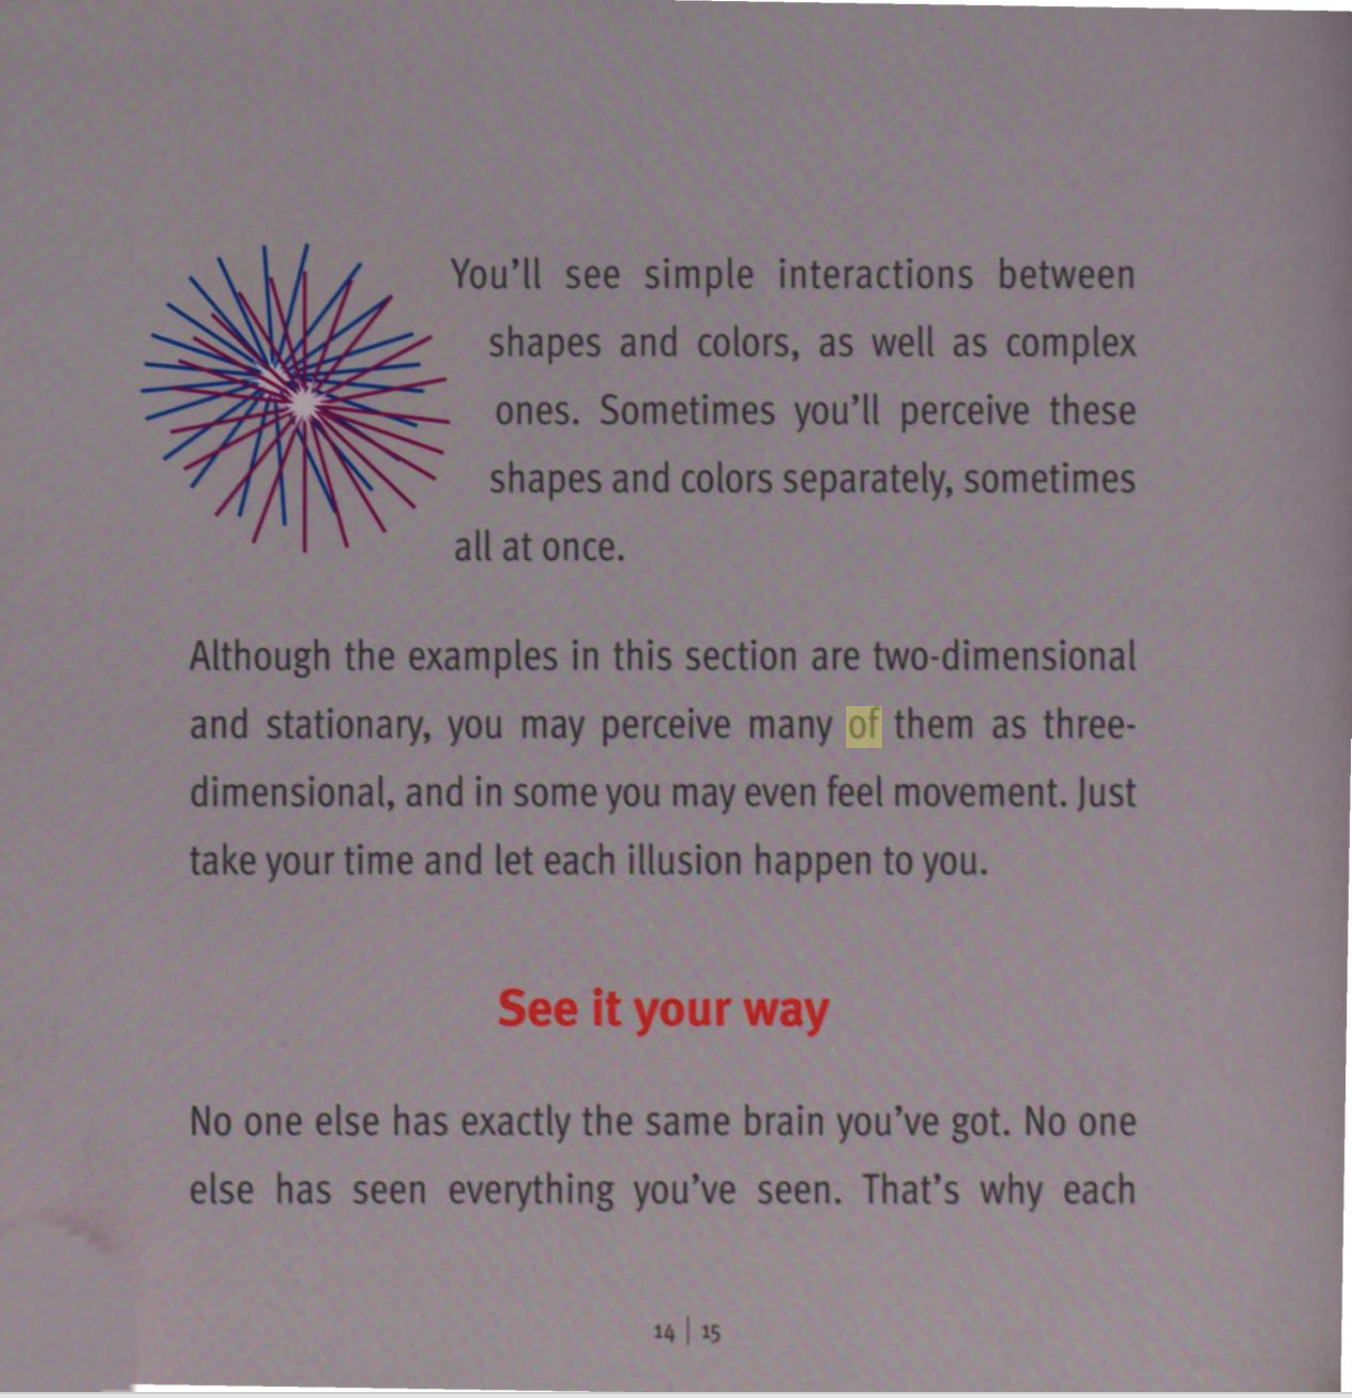
\includegraphics[width=0.6 \linewidth]{./img/bad-illusion.png} 
    \caption{A (digital) example of an illusion which doesn't work after it's
    explained}\label{fig:illusion}
\end{figure}

While walking upstairs to bed yesterday, I saw a book of optical illusions
\cite{bach2006optical} on
his shelf. This reminded me about the Week 8 material looking at
\textit{Modularity of Mind}.

% Is the mind made up of specialized, independent modules evolved to handle specific tasks, or is it a general-purpose system shaped by experience and learning?

Modularity of mind looks at whether the mind is made of specialised, independent
modules evolved to handle specific tasks or whether its a single general-purpose
system.

The book of optical illusions had many interesting illusions. Some illusions
were like the M\"{u}ller-Lyer illusion: even when I knew what the ``trick'' was,
I still couldn't force myself to see it. 

However, others (such as that shown in Figure \ref{fig:illusion}) were easier to
rationalise once you understood what was going on. I first saw the illusion as
being three-dimensional, but after reading the prose on the page, only see it in
two dimensions.

I wondered whether this could be a counterexample to encapsulation, but then I
thought it more easily explained by a somewhat bad optical illusion.

\bibliographystyle{vancouver}
\bibliography{illusions}

\end{document}


